\aufgabe 1

\subsection*{Derivates}
\begin{figure}[h]
	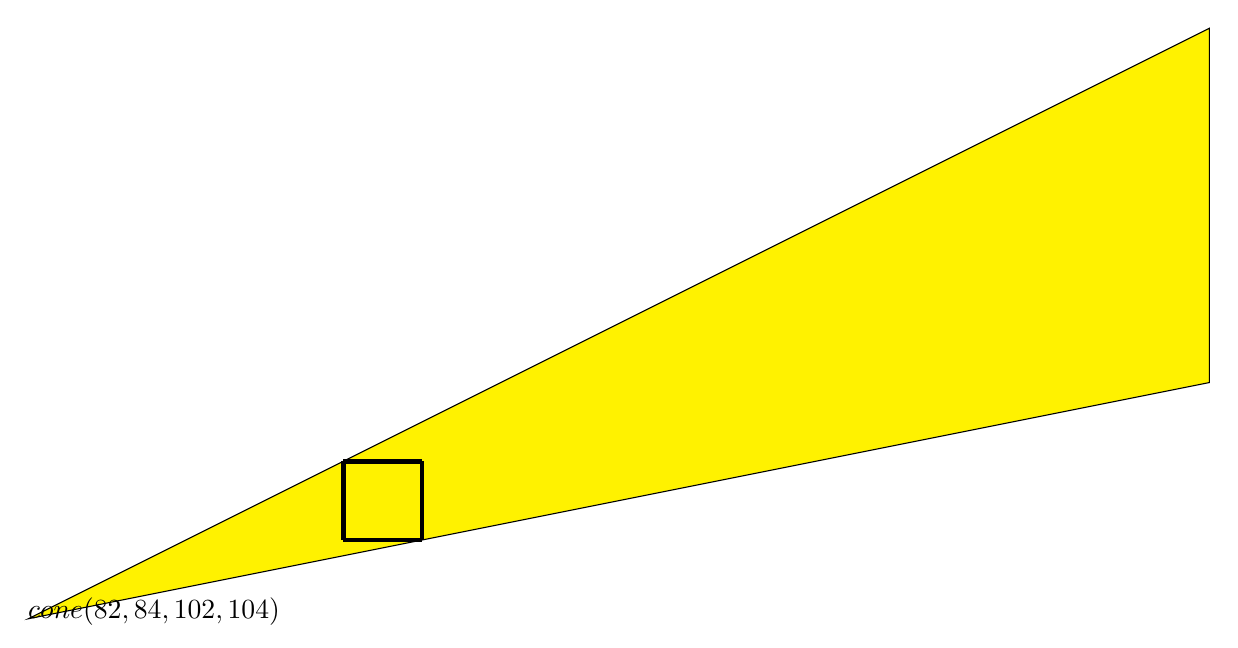
\begin{tikzpicture}[scale=0.5]
	\tkzInit[xmax=30,ymax=15,xmin=0,ymin=0]
	\tkzGrid
	\tkzAxeXY
	\draw[fill=yellow] (30,15) -- (0,0) -- (30,6) -- cycle;
	\draw[line width = 0.6mm] (8,2) -- (8,4) node[] {};
	\draw[line width = 0.6mm] (8,2) -- (10,2) node[] {};
	\draw[line width = 0.6mm] (10,2) -- (10,4) node[] {};
	\draw[line width = 0.6mm] (8,4) -- (10,4) node[] {};
	\tkzText[below](15,-1){$cone(\Point{8}{2},\Point{8}{4},\Point{10}{2},\Point{10}{4})$}
	\end{tikzpicture}
\end{figure}
\newpage
\subsection*{Time step $l_1$}
\begin{figure}[h]
	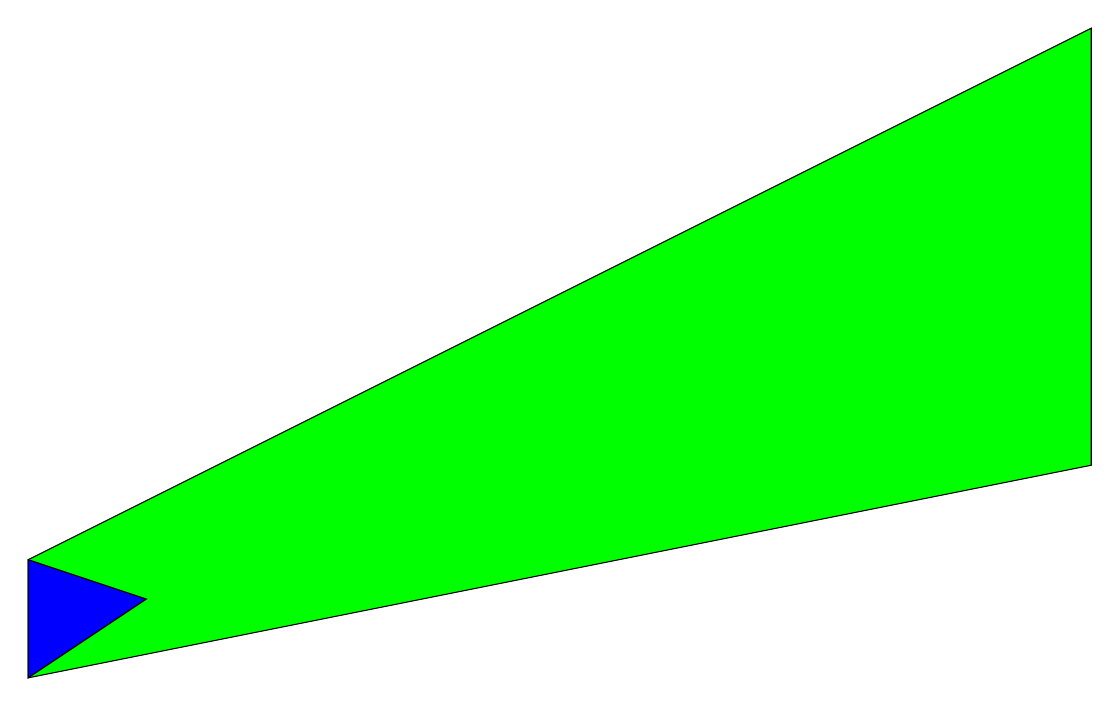
\begin{tikzpicture}[scale=0.5]
	\tkzInit[xmax=30,ymax=20,xmin=0,ymin=0]
	\tkzGrid
	\tkzAxeXY
	\draw[fill=green] (30,18.5) -- (3,5) -- (3,2) -- (30,7.4) -- cycle;
	\draw[fill=blue] (3,2) -- (3,5) -- (6,4) -- cycle;
	\end{tikzpicture}
\end{figure}
\newpage
\subsection*{Invariant Intersection}
\begin{figure}[h]
	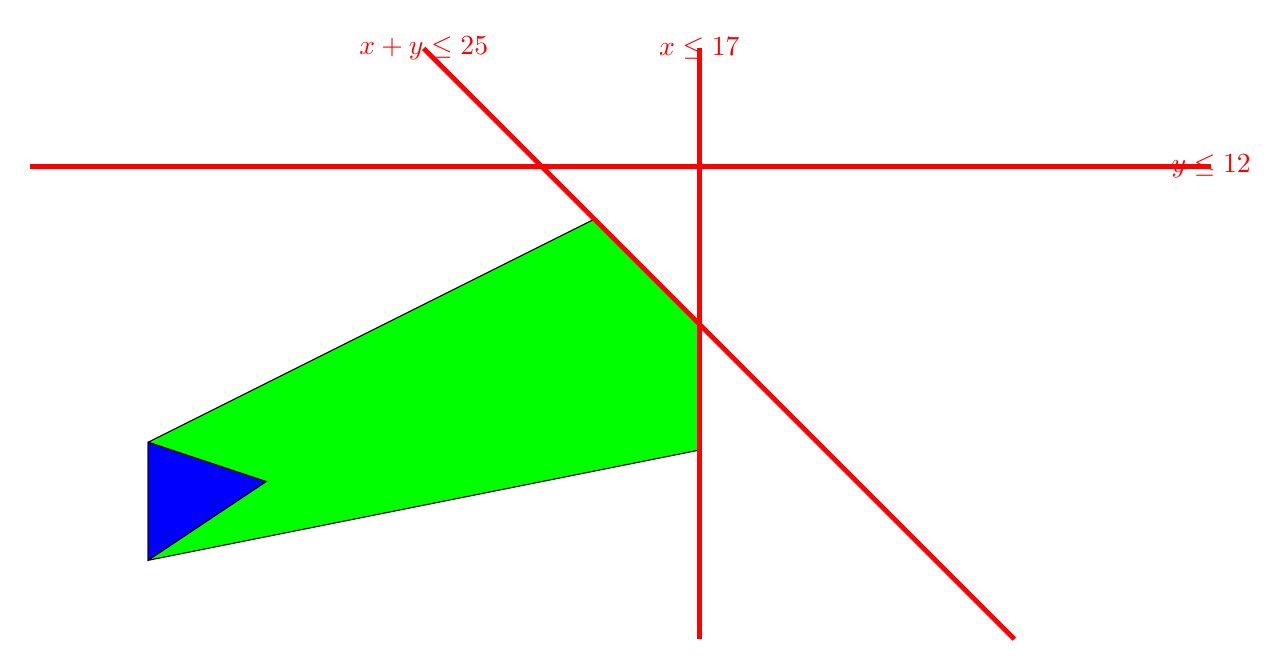
\begin{tikzpicture}[scale=0.5]
	\tkzInit[xmax=30,ymax=15,xmin=0,ymin=0]
	\tkzGrid
	\tkzAxeXY
	\draw[fill=green] (14.333, 10.667) -- (3,5) -- (3,2) -- (17,4.8) -- (17,8) -- cycle;
	\draw[fill=blue] (3,2) -- (3,5) -- (6,4) -- cycle;
	\draw[line width = 0.6mm, color = red] (17,0) -- (17,15) node[] {$x\le 17$};
	\draw[line width = 0.6mm, color = red] (0,12) -- (30,12) node[] {$y\le 12$};
	\draw[line width = 0.6mm, color = red] (25,0) -- (10,15) node[] {$x+y\le 25$};
	\end{tikzpicture}
\end{figure}
\subsection*{Discrete step (guard intersection)}
\begin{figure}[h]
	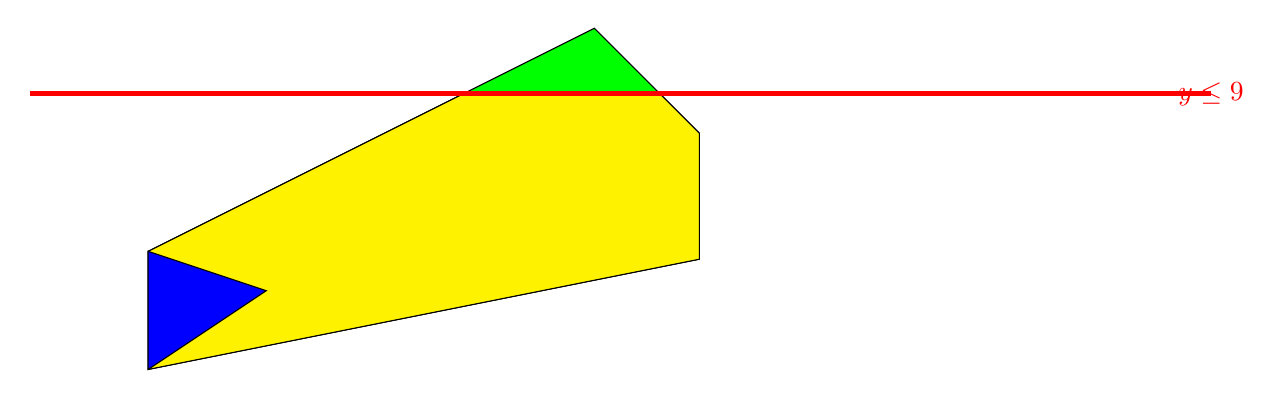
\begin{tikzpicture}[scale=0.5]
	\tkzInit[xmax=30,ymax=15,xmin=0,ymin=0]
	\tkzGrid
	\tkzAxeXY
	\draw[fill=green] (14.333, 10.667) -- (3,5) -- (3,2) -- (17,4.8) -- (17,8) -- cycle;
	\draw[fill=yellow] (11,9) -- (3,5) -- (3,2) -- (17,4.8) -- (17,8) -- (16,9) -- cycle;
	\draw[fill=blue] (3,2) -- (3,5) -- (6,4) -- cycle;
	\draw[line width = 0.6mm, color = red] (0,9) -- (30,9) node[] {$y\le 9$};
	\end{tikzpicture}
\end{figure}
\newpage
\subsection*{Discrete step (reset function)}
\begin{figure}[h]
	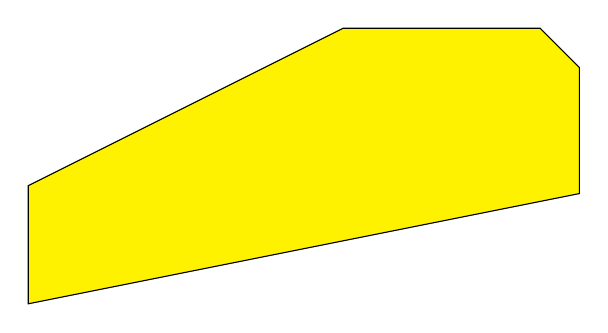
\begin{tikzpicture}[scale=0.5]
	\tkzInit[xmax=30,ymax=20,xmin=0,ymin=0]
	\tkzGrid
	\tkzAxeXY
	\draw[fill=yellow] (11,18) -- (3,14) -- (3,11) -- (17,13.8) -- (17,17) -- (16,18) -- cycle;
	\end{tikzpicture}
\end{figure}